% Lecture file created by Gemini
% Class: Quantum Information With Atoms and Photons
% Professor: Pietro Silvi
% Date: 2025-10-16
\lecture{7}{Lamb-Dicke Regime}{2025-10-16}

% --- Start writing here ---
\captionsetup{singlelinecheck=false}
optically-coupling electronic levels WITH CENTER-OF-MASS motion (in a trap) a.ka.\\
the Lamb-Dicke Regime\\
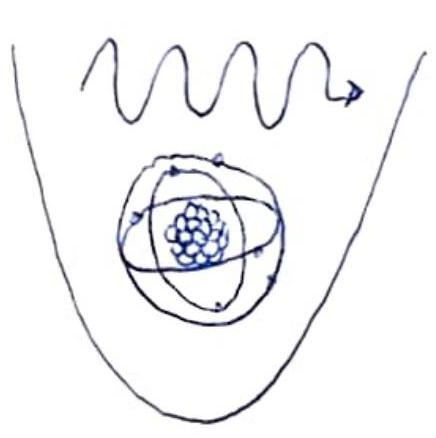
\includegraphics[max=\textwidth, center]{2025_10_16_9146de9f5ba4f09535e7g-1}

3 INGRESIENTS\\
$\rightarrow$ (1.) Hydrogen-Like Atom [Example: $C_{a}^{+}$INO]\\
$\rightarrow$ (2.) Harmonic trap for the center-of-mass motion $\leadsto$ blically in [example; paul trap for lons]\\
$\rightarrow$ (3.) Laser w/ frequency close to optical atomic transitions\\
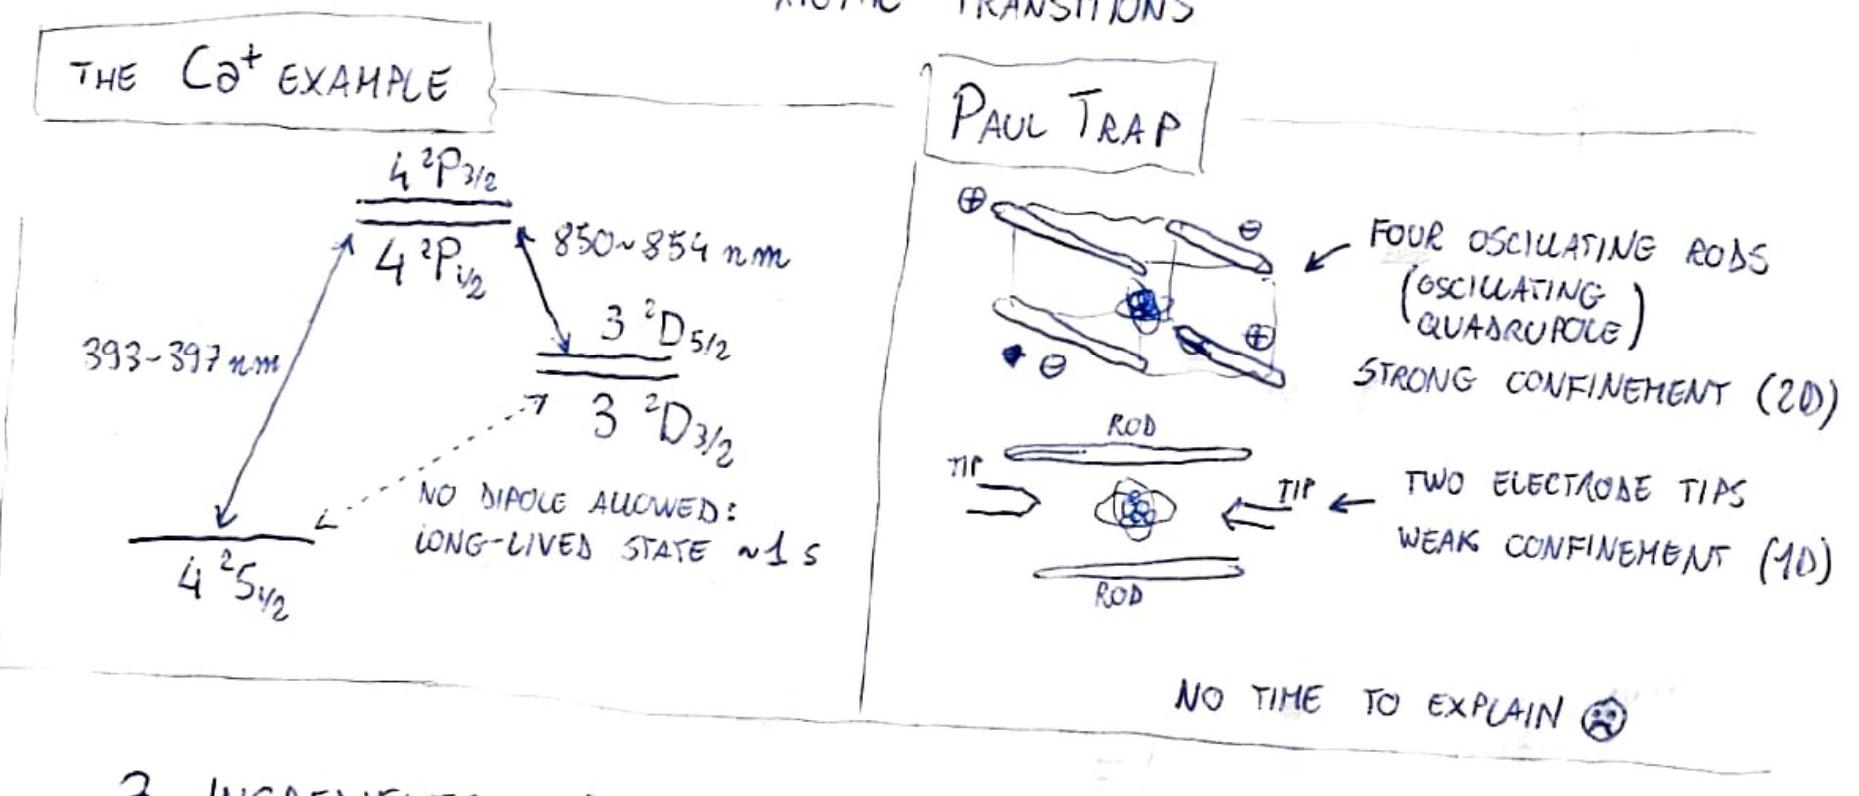
\includegraphics[max=\textwidth, center]{2025_10_16_9146de9f5ba4f09535e7g-1(1)}\\
3. INGREDIENTS $\Rightarrow 3$ LENGEMSCALES!\\
(1.) typical atomic

RASIUS = TYPICAL "BOMR RASIUS" OF relative coorsinate $\approx$ the outer electron OF OUTER ELECTRON

HYARO BOUR RAA.\\
$\tilde{a}_{0} \approx \frac{\left(n^{2}\right)}{Z_{\text {ell }}} \stackrel{\downarrow}{a_{0}}=\frac{n^{2}}{Z_{2}} \frac{4 \pi \varepsilon_{0} \hbar}{\frac{m e^{2}}{4 \text { Rescees }}} \leqslant 1_{n m}$

$$
\int_{n=4(45)}^{\left.\left(C \partial^{+}\right) \rightarrow(4)^{2}\right)} p m \approx 0,42
$$

(3.) CASER WAVELENGTH $\lambda_{\text {LASER }}=\frac{2 \pi \mathrm{C}}{\omega_{L}}$ or $\begin{gathered}\text { FOR OPTICAL TRANSITIONS } \\ \lambda \approx 100 \mathrm{~nm} \sim 1 \mu \mathrm{~mm} \\ (\mathrm{UV})\end{gathered}$ (IR) $\overbrace{\text { Ca+ TRINSITIONS }}^{400 \mathrm{~nm} ; 850 \mathrm{~nm}}$\\
first lenghtscale SEPARATION\\
$\tilde{a}_{0} \ll \lambda \leftarrow\left[\begin{array}{l}\text { atoms are shauer than the wavelengths } \\ \text { of iasers that excite them (harco usea this) }\end{array}\right.$\\
(20)\\
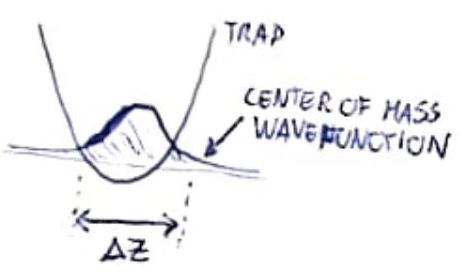
\includegraphics[max=\textwidth, center]{2025_10_16_9146de9f5ba4f09535e7g-2}

$$
\begin{aligned}
& \text { TRAPPING } \\
& \text { POTENTIAL }
\end{aligned} V\left(z_{C, M_{0}}\right)=\frac{1}{2} m_{A} \omega_{\text {TRAP }}^{2} z^{2} \quad\binom{\text { UARAONIC }}{\text { APPRCX. }}
$$

\begin{center}
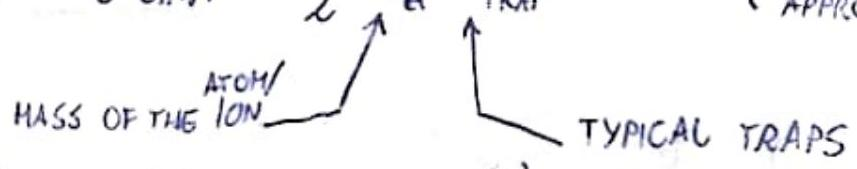
\includegraphics[width=0.5\textwidth]{2025_10_16_9146de9f5ba4f09535e7g-2(1)}
\end{center}

$$
m_{\mathrm{Ca}^{+}} \approx 40 \mathrm{~m}_{\text {PROTON }} \quad \frac{\omega}{2 \pi}=0.1 \sim 10 \mathrm{MHz}
$$

ASSUMING THAT THE CENTER-OF-MASS IS IN THE GROUND TATE OF THE HARMONIC OUCIUATOR

$$
H=\frac{P^{2}}{2 m_{A}}+\frac{m_{A} \omega_{T}^{2}}{2} z^{2}=\hbar \omega_{T}\left(a^{+} a+\frac{1}{2}\right)
$$

$$
\begin{aligned}
& Q z=\sqrt{\frac{\hbar}{2 m_{A} \omega_{T}}}\left(a+a^{+}\right) \quad P=\sqrt{\frac{\hbar m_{A} \omega_{T}}{2}} i\left(a^{+}-a\right) \quad \text { outcomes } \\
&\langle 0| z|0\rangle=\sqrt{\frac{\hbar}{2 m_{A} \omega_{T}}}\left(\langle\phi\rangle+\left\langle\phi^{+}\right\rangle\right)=0 \\
& \Delta z=\sqrt{\langle 0| z^{2}|0\rangle-\langle z\rangle^{-}}=\sqrt{\left(\frac{\hbar}{2 m_{A} \omega_{T}}\right)\left(\left\langle\phi^{*}\right\rangle+\left\langle a^{+} a\right\rangle+\left\langle a a^{+}\right\rangle+\left\langle\phi^{+}\right\rangle\right)} \\
& \Delta z=\sqrt{\frac{\hbar}{2 m_{A} \omega_{T}}}=\sqrt{\frac{(2 \pi \hbar)}{2 m_{A}\left(\frac{\omega_{T}}{2 \pi}\right)}}=\sqrt{\frac{10^{-34} k_{G} m^{2} s^{-2}}{2 \cdot 40 \cdot\left(1.66 \cdot 10^{-27} k_{g}\right)\left[10^{+\frac{1}{2}} \sim 10^{+7} s^{-1}\right]}} \\
&=\sqrt{\left[10^{-16} \sim 10^{-14} m^{2}\right.}=10^{-8} \sim 10^{-7} \mathrm{~m}=10400
\end{aligned}
$$

SECOND LENGHTSCALE SEPARATION?

\begin{displayquote}
BUT NOT TOO SHALL $(\cos \theta)$
\end{displayquote}

is the fitom position fixes at the laser wavelength?\\
tunable via trapting FREQUENCY

I CAN NOW USE $\eta$ AS A SHALL PARAMETER and carry out expansions. hahictonians.\\
$H_{\substack{\text { REATIVE } \\ \text { COODINATE }}}^{\substack{\text { ATOM } \\ \text { REATE }}}=\hbar \omega_{\text {eg }}|e \times e|$\\
$H_{\substack{\text { CENTER-GFASS } \\ \text { COORDINATE }}}^{\text {TOM }}=\hbar \omega_{\text {TRAP }} a^{+} a\binom{\text { FORGET THE }}{+\frac{1}{2} \text { CONTANT }} \leftarrow \begin{gathered}\text { ATOM COM VIBRATIONS } \\ \text { "PHONONS" }\end{gathered}$\\
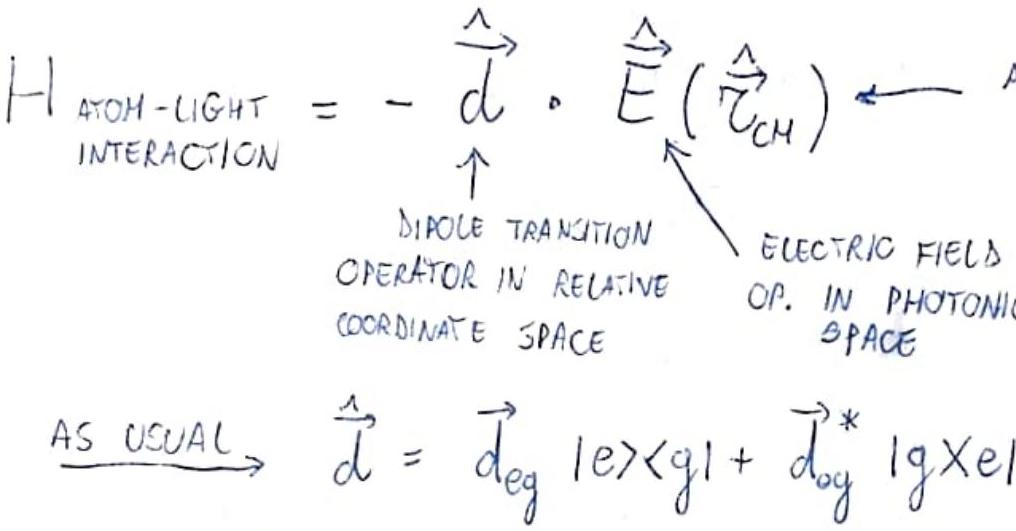
\includegraphics[max=\textwidth, center]{2025_10_16_9146de9f5ba4f09535e7g-3(1)}\\
$\hat{\vec{E}}=\sum_{k \lambda} \sqrt{\frac{\hbar \omega_{k}}{2 \varepsilon_{0}}} \vec{\epsilon}_{k \lambda} 2 \operatorname{Im}\left(u_{k \lambda}\left(\hat{\vec{r}}_{k+1}\right) \hat{a}_{k \lambda}\right)$ LASER IN $|0\rangle|0\rangle|0\rangle \ldots|\alpha\rangle|0\rangle \ldots$ $k \lambda$\\
$\left\langle\psi_{C HS E R}\right| \hat{\vec{E}}\left|\psi_{W S E R}\right\rangle(\hat{\vec{r}})=\ldots=\vec{\xi} \cos (|\overrightarrow{\vec{k}}| t-\overrightarrow{\vec{k}} \cdot \hat{\vec{r}})$ Totile an operator polnt: IN THE COM coordinate

\begin{figure}[h]
\begin{center}
  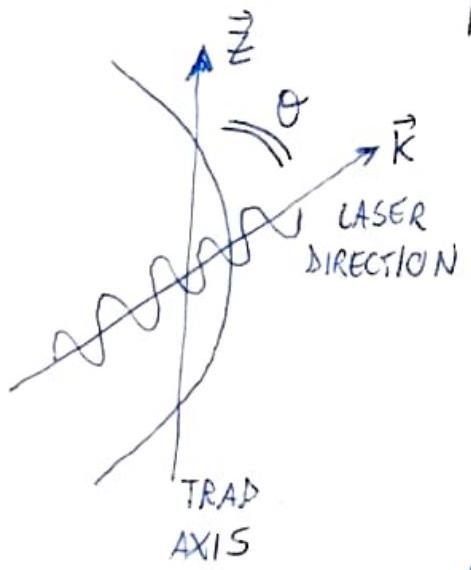
\includegraphics[width=\textwidth]{2025_10_16_9146de9f5ba4f09535e7g-3}
\captionsetup{labelformat=empty}
\caption{INTERNAL STATES}
\end{center}
\end{figure}

trap is tight IN XY 50 ATOM COM COORDINATE OPERATOR

HERE I AMUSING $\tilde{a}_{0} \ll \Delta z_{0}$ IN PH\\
SPACE $\_\_\_\_$ $k \lambda (0) \longleftarrow$ NO MOTION ALLOWES

$$
\langle\vec{E}\rangle(\hat{\vec{r}})=\vec{\xi} \cos (c|\vec{k}| t-\cos \theta|\vec{k}| z)
$$

as usual $\Omega=\frac{\vec{d}_{\text {ey }} \cdot \vec{\xi}}{\hbar}$ rabi frequency $\operatorname{ligm}_{\substack{\text { ITGH } \\ \text { LIGH }}}=-\hbar \Omega|e \times g| \cos (c k t-k \hat{z} \cos \theta)+h . c$. 1 CAN CHANGE THIS SIGN $U=\left(\begin{array}{ll}1 & |e\rangle \\ -1 & |g\rangle\end{array}\right. |e\rangle \rightarrow-|e\rangle$

NEW TERM FROM LAST TIME THE laser actuauy couples RELATIVE $\longleftrightarrow$ COM

$$
H_{\text {rou }}^{(\text {IAB })}=\underset{\substack{\lambda \\ \text { AOUE } \\ \text { CVELS }}}{\hbar \omega_{\text {ey }}}|e \times e|+\underset{\substack{R A P \\ \text { TEVELS }}}{\hbar \omega_{\tau} c^{+} a}+\underset{\substack{R \\ R A B \mid}}{\hbar \Omega}|e \times g| \cos (c K t-K z \cos \theta)+h, c .
$$

$$
\Omega, \Delta \leqslant \omega_{\text {eg }}, \omega_{L}
$$

$\left.H_{\text {FUL }}^{\binom{\text {Rotal }}{\text { RRAME }}}=\hbar\left(\omega_{\text {eg }}-\omega_{L}\right) \right\rvert\,$ exel $\left.+\hbar \omega_{\tau} a^{+} a+\frac{\hbar \Omega}{2} \right\rvert\,$ exgl $e^{-i \cos \theta k \hat{z}}+$ h.c.\\
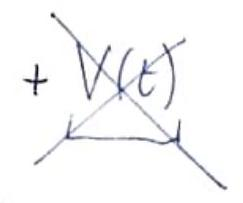
\includegraphics[max=\textwidth, center]{2025_10_16_9146de9f5ba4f09535e7g-4(2)}

BUT\\
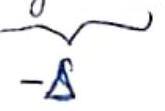
\includegraphics[max=\textwidth, center]{2025_10_16_9146de9f5ba4f09535e7g-4(3)}\\
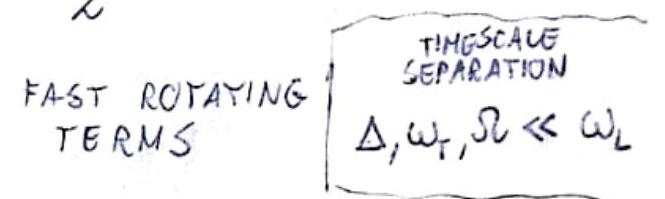
\includegraphics[max=\textwidth, center]{2025_10_16_9146de9f5ba4f09535e7g-4}

$$
\begin{aligned}
\cos \theta K \hat{z} & =1 K \cos \theta \sqrt{\frac{\hbar}{2 m_{A} \omega_{T}}}\left(a+a^{+}\right)=(\Delta Z K \cos \theta)\left(a+a^{+}\right) \\
& =\eta\left(a+a^{+}\right) \quad \text { AMA!! AND } \eta \text { SHALU PARAMETER }
\end{aligned}
$$

$$
e^{-i \cos \theta k \hat{z}}=e^{-i \eta\left(a+a^{+}\right)}=1-i \eta\left(a^{+}+a\right)+\theta\left(\eta^{2}\right)
$$

$H_{\text {FULC }}^{\text {(eotc) }}=\underbrace{\hbar \omega_{7} a^{+} a}_{\text {ONCY INTERNAL }} \cdot \underbrace{\hbar \Delta|e \times e|+\frac{\hbar \Omega}{2}(|e \times y|+|g \times e|)}_{\substack{\text { ONCY } \\ \text { PHONON }}}+$

LAMS-DICKE

$$
+\eta \frac{\hbar \Omega}{2}(-i \underbrace{|\overrightarrow{e xg}|+i \mid \overrightarrow{g x}(\vec{x} \mid}_{\sigma^{y}})\left(a^{+}+a\right)
$$

$H_{\text {FUll }}^{(\text {eoil })}=\hbar \omega_{T} a^{+} a-\hbar \Delta|e x e|+\frac{\hbar \Omega}{2} \sigma^{X}+\eta \frac{\hbar \Omega}{2} \sigma^{Y}\left(a^{+}+a\right)$ NICE\\
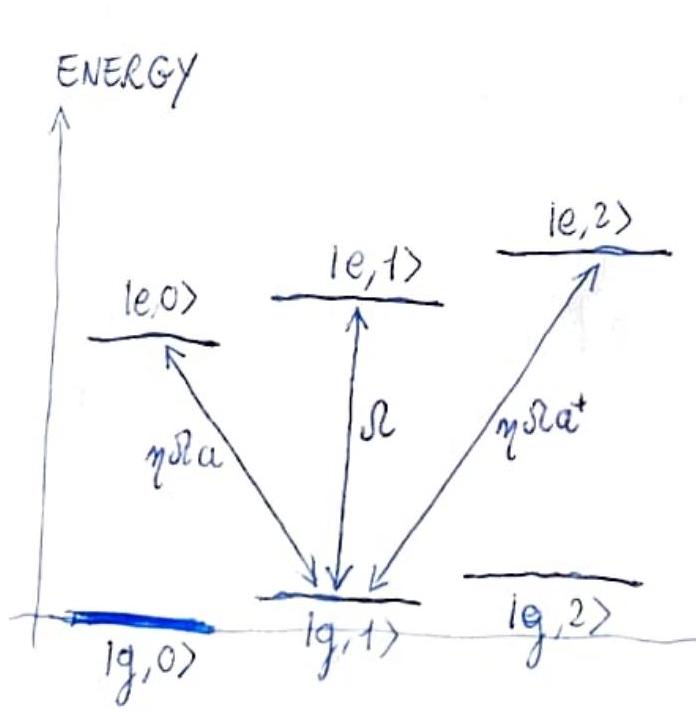
\includegraphics[width=0.5\textwidth, center]{2025_10_16_9146de9f5ba4f09535e7g-4(1)}

$$
\begin{array}{|lr}
\hline \Omega=0 & \text { BARE SPECTROM } \\
\hline \omega_{L}=0 & \\
& \begin{array}{l}
\text { I THEN TURN } \\
\text { THE LASER ON }
\end{array}
\end{array}
$$

ig,n) couples to $\left\langle\begin{array}{l}\langle i, n-i\rangle \\ |e, n\rangle \\ |e, n+1\rangle\end{array}\right.$

$$
3 \text { (SUB)-REGMES }
$$

phonows\\
(1) CARRIER RESONANCE\\
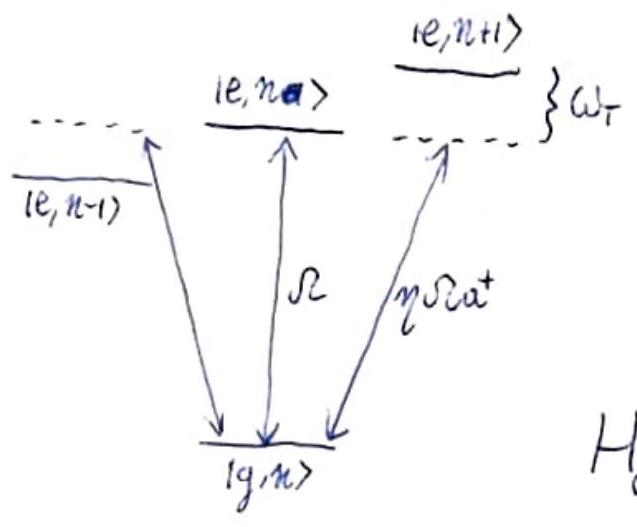
\includegraphics[width=0.5\textwidth, center]{2025_10_16_9146de9f5ba4f09535e7g-5(3)}\\
iaser in resonant with the drect transition $\Delta \ll \omega_{T} \quad\left(\right.$ AND WEAK $\left.\eta \Omega \ll \omega_{T}\right)$\\
$|g, n\rangle ;|e, n \pm 1\rangle \rightarrow$ haterx ecement $q \Omega$\\
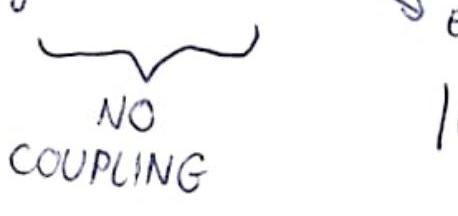
\includegraphics[width=0.5\textwidth, center]{2025_10_16_9146de9f5ba4f09535e7g-5(4)}\\
ENERGY DIFFERENCE (ROT,)\\
$\left|\omega_{\tau} \pm \Delta\right| \approx \omega_{\tau} \gg \eta \Omega$\\
$H_{\text {CARRER }}=\hbar \omega_{\tau} a^{+} a-\hbar \Delta|e x e|+\frac{\hbar \sigma}{2} \sigma^{x}$\\
(2) RED SIAEBAND\\
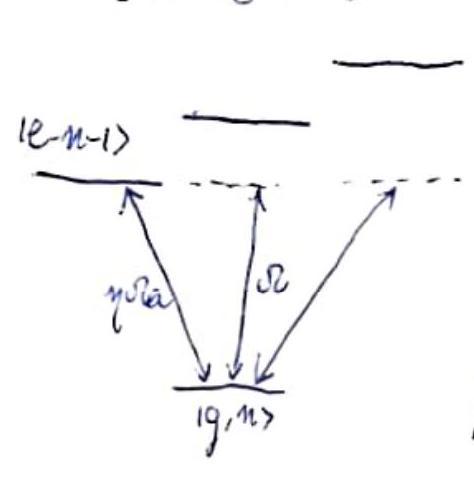
\includegraphics[width=0.5\textwidth, center]{2025_10_16_9146de9f5ba4f09535e7g-5(2)}

Laser $\omega_{L}$ resonant with $\omega_{\text {eg }}-\omega_{T}$, that is\\
$\left|\omega_{L}-\omega_{\text {eg }}+\omega_{T}\right| \leqslant \omega_{T}$\\
$\left|\Delta+\omega_{T}\right| \leqslant \omega_{T} \quad$ (and Weak $\Omega \ll \omega_{T}$ )

$$
\left|\Delta+\omega_{\tau}\right| \leqslant \omega_{\tau}
$$

THEREFORE $|g, n\rangle \stackrel{\text { CNV }}{\longleftrightarrow}|e, n-1\rangle$

$$
\begin{aligned}
& H_{\text {RED }}=\hbar \omega_{T} a^{+} a-\hbar \Delta I|l x e|+\frac{\eta \hbar \Omega}{2}\left(-i|e \times g| a+i|g \times j| a^{+}\right) \\
& =\hbar \omega_{T} a^{+} a-\hbar \Delta|e \times e|+\frac{\eta \hbar \Omega}{2}\left(-i \sigma^{+} a+h . c .\right) \\
& \text { JAYNES-CUMMINGS MODEL (BETWEEN PHONON AND CEVEL) }
\end{aligned}
$$

laser detunes to lower ("res") frequencies than carrer\\
(3) BLUE SIDEBAND\\
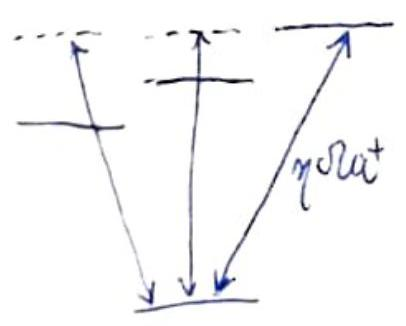
\includegraphics[width=0.5\textwidth, center]{2025_10_16_9146de9f5ba4f09535e7g-5}\\
$\omega_{L}$ resonant with $\omega_{\text {eg }}+\omega_{T}$, or\\
$\left|\omega_{L}-\omega_{\text {eg }}-\omega_{T}\right| \leqslant \omega_{T} \quad$ (and ofc. $\Omega \ll \omega_{T}$ ) $\left|\Delta-\omega_{g}\right| \leqslant \omega_{\tau}$\\
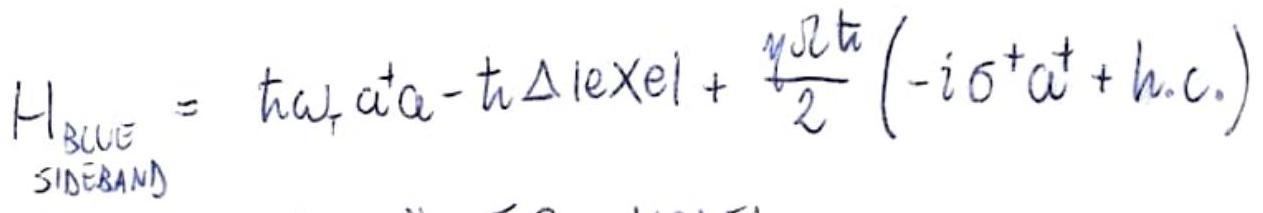
\includegraphics[width=0.5\textwidth, center]{2025_10_16_9146de9f5ba4f09535e7g-5(1)} "ANTI"-JC MODEL

\begin{figure}[h]
\begin{center}
  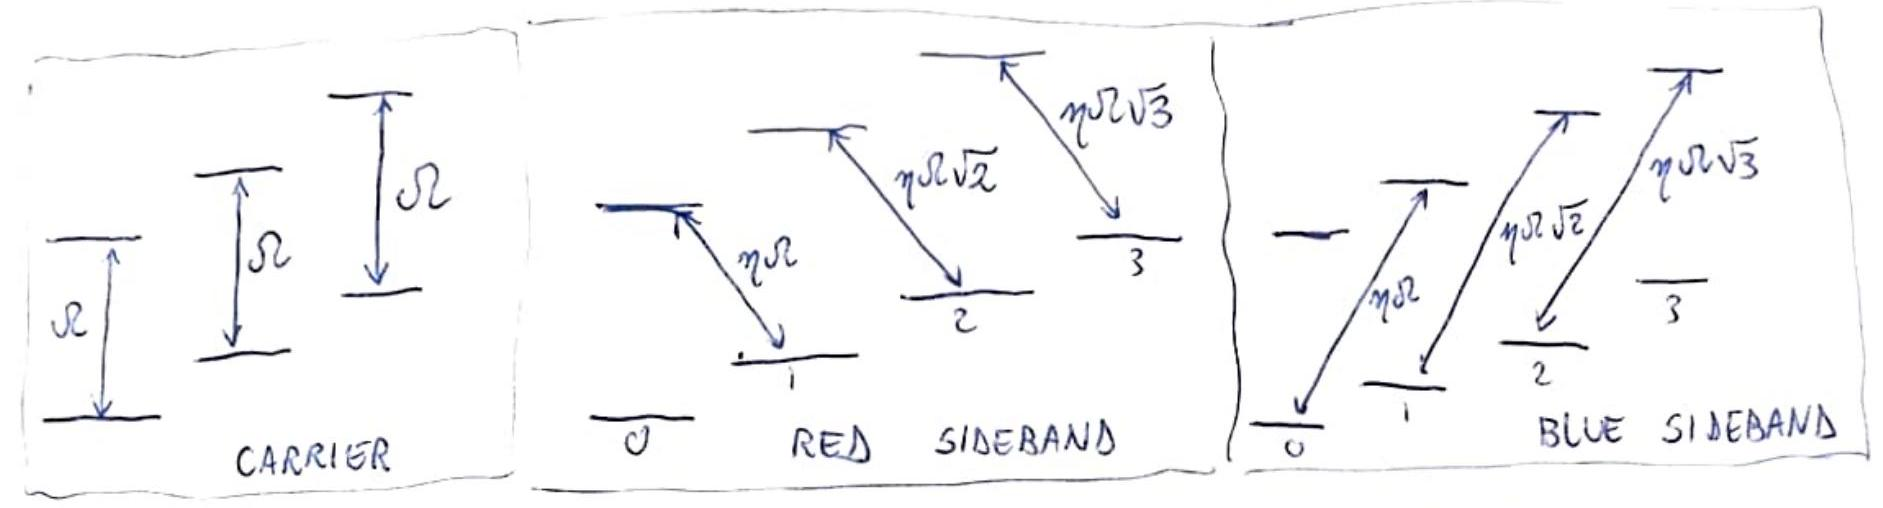
\includegraphics[width=\textwidth]{2025_10_16_9146de9f5ba4f09535e7g-6(1)}
\captionsetup{labelformat=empty}
\caption{EFF. FREQUENCIES MATCH}
\end{center}
\end{figure}

$$
1 \mathrm{MHz}=\overbrace{48 \mu \mathrm{~K}}^{\text {THAT'S FRIGGHN }}
$$

$\left\{\begin{array}{l}\text { EFF. FREQUENCIES MISMATCH } \\ \text { AND INCOMMENSURATE!! } \\ \text { THIS IS AN ISSUE WHEN IESIGNING }\end{array}\right.$\\
THIS IS AN ISSUE WHEN DESIGNING multi-qubit gates on ion trads: ASYNCHRONY REQURES PERFECT COCLING OR WORKAROUND

BTW, the red sideband can be used to cool-down atom vibrations\\
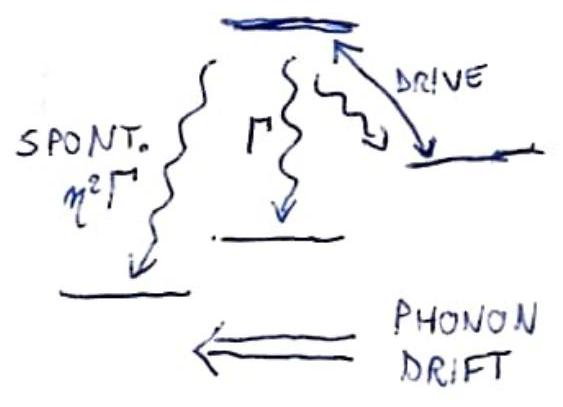
\includegraphics[width=0.5\textwidth, center]{2025_10_16_9146de9f5ba4f09535e7g-6}
